\begin{figure}[H]
    \centering
    \begin{minipage}[c][8.3cm][c]{0.28\textwidth}
        \centering
        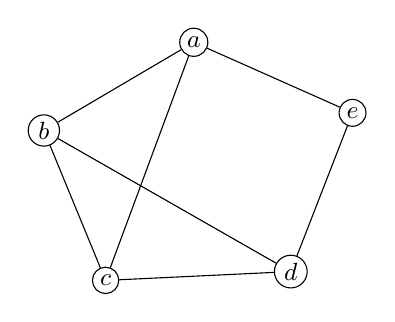
\begin{tikzpicture}[scale=1.12,every node/.style={circle,draw,inner sep=1.4pt,font=\small}]
            \node (a) at (0.0,1.4) {$a$};
            \node (b) at (-1.7,0.4) {$b$};
            \node (c) at (-1.0,-1.3) {$c$};
            \node (d) at (1.1,-1.2) {$d$};
            \node (e) at (1.8,0.6) {$e$};

            \draw (a) -- (b);
            \draw (a) -- (c);
            \draw (a) -- (e);
            \draw (b) -- (c);
            \draw (c) -- (d);
            \draw (b) -- (d);
            \draw (d) -- (e);
        \end{tikzpicture}
        \\\smallskip
        {\small Input graph $G$.}
    \end{minipage}
    \hfill
    \begin{minipage}[c][8.3cm][c]{0.68\textwidth}
        \centering
        \begin{tikzpicture}[
            x=1.15cm,
            y=1.15cm,
            every node/.style={circle,draw,inner sep=1.2pt,font=\scriptsize},
            base/.style={circle,draw,fill=white,inner sep=1.2pt,font=\scriptsize},
            tnode/.style={circle,draw=cutD,fill=cutD!25,inner sep=1.1pt,font=\scriptsize,transform shape=false},
            tedge/.style={draw=cutD,very thick}
        ]
            \coordinate (a) at (0.0,1.2);
            \coordinate (b) at (-1.6,0.45);
            \coordinate (c) at (-1.0,-1.15);
            \coordinate (d) at (0.95,-1.05);
            \coordinate (e) at (1.7,0.5);

            \draw (a) -- (b);
            \draw (a) -- (c);
            \draw (a) -- (e);
            \draw (b) -- (c);
            \draw (c) -- (d);
            \draw (b) -- (d);
            \draw (d) -- (e);

            % For each vertex v, add an equilateral triangle on {v,v_1,v_2}
            \begin{scope}[shift={(a)}, rotate=90]
                \node[tnode] (a1) at (0.866,0.5) {$a_1$};
                \node[tnode] (a2) at (0.866,-0.5) {$a_2$};
                \draw[tedge] (0,0) -- (a1);
                \draw[tedge] (0,0) -- (a2);
                \draw[tedge] (a1) -- (a2);
            \end{scope}

            \begin{scope}[shift={(b)}, rotate=165]
                \node[tnode] (b1) at (0.866,0.5) {$b_1$};
                \node[tnode] (b2) at (0.866,-0.5) {$b_2$};
                \draw[tedge] (0,0) -- (b1);
                \draw[tedge] (0,0) -- (b2);
                \draw[tedge] (b1) -- (b2);
            \end{scope}

            \begin{scope}[shift={(c)}, rotate=240]
                \node[tnode] (c1) at (0.866,0.5) {$c_1$};
                \node[tnode] (c2) at (0.866,-0.5) {$c_2$};
                \draw[tedge] (0,0) -- (c1);
                \draw[tedge] (0,0) -- (c2);
                \draw[tedge] (c1) -- (c2);
            \end{scope}

            \begin{scope}[shift={(d)}, rotate=312]
                \node[tnode] (d1) at (0.866,0.5) {$d_1$};
                \node[tnode] (d2) at (0.866,-0.5) {$d_2$};
                \draw[tedge] (0,0) -- (d1);
                \draw[tedge] (0,0) -- (d2);
                \draw[tedge] (d1) -- (d2);
            \end{scope}

            \begin{scope}[shift={(e)}, rotate=18]
                \node[tnode] (e1) at (0.866,0.5) {$e_1$};
                \node[tnode] (e2) at (0.866,-0.5) {$e_2$};
                \draw[tedge] (0,0) -- (e1);
                \draw[tedge] (0,0) -- (e2);
                \draw[tedge] (e1) -- (e2);
            \end{scope}

            \node[base] at (a) {$a$};
            \node[base] at (b) {$b$};
            \node[base] at (c) {$c$};
            \node[base] at (d) {$d$};
            \node[base] at (e) {$e$};
        \end{tikzpicture}
        \\\smallskip
        {\small The graph $H$ with triangles attached to each vertex of $G$.}
    \end{minipage}
    \caption{Illustration of the reduction used in Theorem~\ref{thm:hac-inapproximability}. For each original vertex $v\in V(G)$ we add two new vertices $v_1$ and $v_2$ and create the triangle on $\brc{v,v_1,v_2}$.}
    \label{fig:hardness-tree-reduction}
\end{figure}